% Choose one to switch betweeen slides and handout
%\documentclass[]{beamer}
\documentclass[handout]{beamer}

% Video Meta Data
\title{Bitcoin, Blockchain and Cryptoassets}
\subtitle{Economic Scripting}
\author{Prof. Dr. Fabian Schär}
\institute{University of Basel}

% Config File
% Packages
\usepackage[utf8]{inputenc}
\usepackage{hyperref}
\usepackage{gitinfo2}
\usepackage{tikz}
\usepackage{amsmath}
\usepackage{bibentry}
\usepackage{xcolor}
\usepackage{colortbl} % Add colour to LaTeX tables
\usepackage{caption}
\usepackage[export]{adjustbox}
\usepackage{pgfplots} \pgfplotsset{compat = 1.17}

% Color Options
\definecolor{highlight}{rgb}{0.65,0.84,0.82}
\definecolor{focus}{rgb}{0.72, 0, 0}

% Beamer Template Options
\beamertemplatenavigationsymbolsempty
\setbeamertemplate{footline}[frame number]
\setbeamercolor{structure}{fg=black}
\setbeamercolor{footline}{fg=black}
\setbeamercolor{title}{fg=black}
\setbeamercolor{frametitle}{fg=black}
\setbeamercolor{item}{fg=black}
\setbeamercolor{}{fg=black}
\setbeamercolor{bibliography item}{fg=black}
\setbeamercolor*{bibliography entry title}{fg=black}
\setbeamertemplate{items}[square]
\setbeamertemplate{enumerate items}[default]
\captionsetup[figure]{labelfont={color=black},font={color=black}}
\captionsetup[table]{labelfont={color=black},font={color=black}}

\setbeamertemplate{bibliography item}{\insertbiblabel}

% Link Icon Command
\newcommand{\link}{%
    \tikz[x=1.2ex, y=1.2ex, baseline=-0.05ex]{%
        \begin{scope}[x=1ex, y=1ex]
            \clip (-0.1,-0.1)
                --++ (-0, 1.2)
                --++ (0.6, 0)
                --++ (0, -0.6)
                --++ (0.6, 0)
                --++ (0, -1);
            \path[draw,
                line width = 0.5,
                rounded corners=0.5]
                (0,0) rectangle (1,1);
        \end{scope}
        \path[draw, line width = 0.5] (0.5, 0.5)
            -- (1, 1);
        \path[draw, line width = 0.5] (0.6, 1)
            -- (1, 1) -- (1, 0.6);
        }
    }

% Read Git Data from Github Actions Workflow
% Defaults to gitinfo2 for local builds
\IfFileExists{gitInfo.txt}
	{\input{gitInfo.txt}}
	{
		\newcommand{\gitRelease}{(Local Release)}
		\newcommand{\gitSHA}{\gitHash}
		\newcommand{\gitDate}{\gitAuthorIsoDate}
	}

% Custom Titlepage
\defbeamertemplate*{title page}{customized}[1][]
{
  \vspace{-0cm}\hfill
\includegraphics[width=2.5cm]{../config/logo_cif}
  
\includegraphics[width=1.9cm]{../config/seal_wwz}
  \\ \vspace{2em}
  \usebeamerfont{title}\textbf{\inserttitle}\par
  \usebeamerfont{title}\usebeamercolor[fg]{title}\insertsubtitle\par  \vspace{1.5em}
  \small\usebeamerfont{author}\insertauthor\par
  \usebeamerfont{author}\insertinstitute\par \vspace{2em}
  \usebeamercolor[fg]{titlegraphic}\inserttitlegraphic
    \tiny \noindent \texttt{Release Ver.: \gitRelease}\\ 
    \texttt{Version Hash: \gitSHA}\\
    \texttt{Version Date: \gitDate}\\ \vspace{1em}
  \link \href{https://github.com/cifunibas/Bitcoin-Blockchain-Cryptoassets/blob/main/slides/intro.pdf}
  {Get most recent version}\\
  \link \href{https://github.com/cifunibas/Bitcoin-Blockchain-Cryptoassets/blob/main/slides/intro.pdf}
  {Watch video lecture}\\ \vspace{1em}
  License: \texttt{Creative Commons Attribution-NonCommercial-ShareAlike 4.0 International}\\\vspace{2em}
  
\includegraphics[width = 1.2cm]{../config/license}
}

% tikzlibraries
\usetikzlibrary{decorations.pathreplacing}
\usetikzlibrary{decorations.markings}
\usetikzlibrary{positioning}

%caption font
\captionsetup{font=footnotesize}


% Other Inputs
% Defining Bitcoin Symbol
\def\btc{%
	\leavevmode
	\vtop{\offinterlineskip %\bfseries
		\setbox0=\hbox{B}%
		\setbox2=\hbox to\wd0{\hfil\hskip-.03em
			\vrule height .3ex width .15ex\hskip .08em
			\vrule height .3ex width .15ex\hfil}
		\vbox{\copy2\box0}\box2}}
% Definition of a green checkmark symbol
% Code based on: https://tex.stackexchange.com/questions/532033/make-a-double-blue-checkmark-symbol-with-square-contours-using-tikz

% Create shape of a green checkmark
\tikzset{pics/.cd, checkmark/.style={code={% 
			\pgfgettransformentries{\tmpxx}{\tmp}{\tmp}{\tmp}{\tmp}{\tmp}
			\draw[line width=\tmpxx*1pt,draw=none,fill=green!60] (0,.33) -- (.25,0) to 
			(0.8,.6) to (.72,.68) to (.25,.18) to (0.08,.40)-- cycle;}}}

\newcommand{\checkmarkgreen}{
\begin{tikzpicture}[baseline={(0,0)}]
		\path (0,0) pic[scale=1]{checkmark};
\end{tikzpicture}}



%%%%%%%%%%%%%%%%%%%%%%%%%%%%%%%%%%%%%%%%%%%%%%
%%%%%%%%%%%%%%%%%%%%%%%%%%%%%%%%%%%%%%%%%%%%%%
\begin{document}

\thispagestyle{empty}
\begin{frame}[noframenumbering]
	\titlepage
\end{frame}

%%%

\begin{frame}{Transactions Review}
	What has been covered so far:
	\begin{itemize}
		\item<1 -> Transaction types
		\begin{itemize}
			\item<1 -> Pay-to-Address, Pay-to-Multisig, Pay-to-Script-Hash, etc.
		\end{itemize}
		\item<2 -> Signature hash types
		\begin{itemize}
			\item<2 -> \texttt{SIGHASH\_ALL}, \texttt{SIGHASH\_NONE|SIGHASH\_ANYONECANPAY}, etc.
		\end{itemize}
		\item<3 -> Using these components and clever transaction design, smart contracts can be implemented on the Bitcoin Blockchain.
	\end{itemize}
\end{frame}

%%%

\begin{frame}{Example: Conditional Purchase Agreement}
	\begin{figure}[h]
		\begin{minipage}{0.2\linewidth}
			\centering
			
\includegraphics[width=1cm]{../assets/images/agents/handing_right}
			\begin{tikzpicture}[overlay]
				\node at (-0.05,0.18) {
\includegraphics[width = 0.5cm]{../assets/images/bitcoin}};
			\end{tikzpicture}
		\end{minipage}%
		\begin{minipage}{0.15\linewidth}
			\centering
			\vspace{-2cm}
			\only<3>{
\includegraphics[width=1cm]{../assets/images/agents/intermediary_devil}}
		\end{minipage}%
		\begin{minipage}{0.25\linewidth}
			\centering
			
\includegraphics[width=1cm]{../assets/images/agents/handing_left}
			\begin{tikzpicture}[overlay, coloredCoin/.style={circle,  very thick, minimum size=0.5mm}]
				\node[coloredCoin, draw=orange!60, fill=orange!5] at (-1.5,0.9) {\footnotesize{$\btc$}};
			\end{tikzpicture}
		\end{minipage}
	\end{figure}
	\begin{itemize}
		\item<1 ->Goal: Alice wants to purchase a colored coin from Bob.
		\item<2 ->Issue: None of the two wants to transfer their asset first.
		\item<3 ->Traditionally, centralized service would be used. But they can potentially be malicious and/or costly.
		\item<4 ->Using an elegant transaction design, they can do the transaction on-chain and trustless.
	\end{itemize}
\end{frame}

%%%

\begin{frame}{Conditional Purchase Agreement: Transaction Details}
	\begin{figure}
			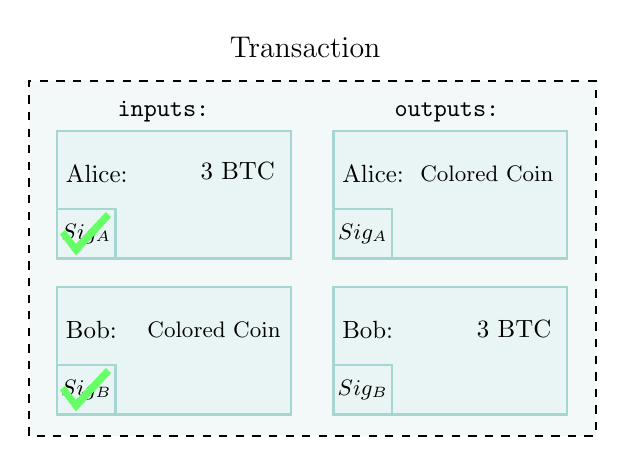
\begin{tikzpicture}[scale=0.9, every node/.style={scale=0.9}]
				\filldraw[yshift=-0.05cm, xshift=0.1cm,color = highlight!15, thick, 	draw=black, dashed] (-3,-5.9) rectangle ++(8cm,5cm);
				
				\draw[color=black] plot (1,-0.2) node [below]
				{\large{{Transaction}}};
				
				% Inputs
				\draw[color=black] plot (-1,-1.65) node[above] {\texttt{inputs:}};
				
				% top left
				\filldraw[yshift=-0.05cm, xshift=0.1cm,color = highlight!25, thick, 	draw=highlight] (-2.6,-3.4) rectangle ++(3.3cm,1.8cm);
				\filldraw[yshift=-0.05cm, xshift=0.1cm,color = highlight!25, thick, 	draw=highlight] (-2.6,-3.4) rectangle ++(0.825cm,0.7cm);
				\draw[color=black] plot (-2.5,-2.25) node[right] {Alice:};
				\draw[color=black] plot (-0.6,-2.21)   node[right] {3 BTC};
				\draw[color=black] plot (-2.0875,-3.1)   node {\small{$Sig_A$}};
			
				\uncover<2 ->{\draw plot (-2.1,-3.1) node {\checkmarkgreen};}
						
				% bottom left
				\uncover<3->{
				\filldraw[yshift=-0.05cm, xshift=0.1cm,color = highlight!25, thick, draw=highlight] (-2.6,-5.6) rectangle ++(3.3cm,1.8cm);
				\filldraw[yshift=-0.05cm, xshift=0.1cm,color = highlight!25, thick,draw=highlight] (-2.6,-5.6) rectangle ++(0.825cm,0.7cm);
				\draw[color=black] plot (-2.5,-4.45)   node[right] {Bob:};
				\draw[color=black] plot (-1.35,-4.45)   node[right] {\small{Colored Coin}};
				\draw[color=black] plot (-2.0875,-5.3)   node {\small{$Sig_B$}};}
				
				\uncover<4->{\draw plot (-2.1,-5.3) node {\checkmarkgreen};}
				
				% Outputs
				\draw[color=black] plot (3,-1.65)   node[above] {\texttt{outputs:}};
				
				% top right
				\filldraw[yshift=-0.05cm, xshift=0.1cm,color = highlight!25, thick, draw=highlight] (1.3,-3.4) rectangle ++(3.3cm,1.8cm);
				\filldraw[yshift=-0.05cm, xshift=0.1cm,color = highlight!25, thick, 	draw=highlight] (1.3,-3.4) rectangle ++(0.825cm,0.7cm);
				\draw[color=black] plot (1.4,-2.25)   node[right] {Alice:};
				\draw[color=black] plot (2.5,-2.25)   node[right] {\small{Colored Coin}};
				\draw[color=black] plot (1.8125,-3.1)   node {\small{$Sig_A$}};
				
				% bottom right
				\filldraw[yshift=-0.05cm, xshift=0.1cm,color = highlight!25, thick, draw=highlight] (1.3,-5.6) rectangle ++(3.3cm,1.8cm);
				\filldraw[yshift=-0.05cm, xshift=0.1cm,color = highlight!25, thick,draw=highlight] (1.3,-5.6) rectangle ++(0.825cm,0.7cm);
				\draw[color=black] plot (1.4,-4.45)   node[right] {Bob:};
				\draw[color=black] plot (3.3,-4.45)   node[right] {3 BTC};
				\draw[color=black] plot (1.8125,-5.3)   node {\small{$Sig_B$}};
		\end{tikzpicture}
	\end{figure}
	\begin{itemize}
		\item<1 ->Alice creates "wrapper" transaction and signs first input  (SIGHASH\_ALL).
		\item<3 ->Bob signs second input (SIGHASH\_ALL).
		\item<4 ->Atomic connection between the two assets' change of ownership. No counterparty risk.
	\end{itemize}
\end{frame}

%%%

\begin{frame}{Further Scripting Components}
	\begin{itemize}
		\item<1-> \textbf{Time Locks}
		\begin{itemize}
			\item<1-> Lock a transaction or output for a relative or absolute point in time.
		\end{itemize}
		\vspace{0.25cm}
		\item<2-> \textbf{Competitive Outputs}
		\begin{itemize}
			\item<2-> Two competing options to use one single output.
		\end{itemize}
		\vspace{0.25cm}
		\item<3-> \textbf{Hash Locks}
		\begin{itemize}
			\item<3-> Require the knowledge of some secret input in order to spend an output.
		\end{itemize}
%		\vspace{0.25cm}
%		\item<4-> Hash Time Locked Contracts
%		\begin{itemize}
%			\item<4-> Create asymmetrically revocable commitments
%		\end{itemize}
	\end{itemize}
\end{frame}

%%%

\begin{frame}{Competitive Outputs}
	\begin{minipage}{0.3\textwidth}
		\begin{figure}
			\begin{tikzpicture}
				[scale=0.9, every node/.style={scale=0.9}]
				% Structure
				\filldraw[yshift=-0.05cm, xshift=0.1cm,color = highlight!15, thick, 	draw=black, dashed] (0.95,-5.8) rectangle ++(4cm,4.9cm);
				\filldraw[yshift=-0.05cm, xshift=0.1cm,color = highlight!25, thick, draw=highlight] (1.3,-5.4) rectangle ++(3.3cm,3.8cm);
				\draw[color=black, thick, dashed] (1.6,-3.75) -- (4.4,-3.75);
				
				% Outputs
				\draw[color=black] plot (3,-1.65)   node[above] {\texttt{outputs:}};
				
				
				% top
				\filldraw[yshift=-0.05cm, xshift=0.1cm,color = highlight!25, thick, 	draw=highlight] (1.3,-3.4) rectangle ++(0.825cm,0.7cm);
				\filldraw[yshift=-0.05cm, xshift=0.1cm,color = highlight!25, thick, 	draw=highlight] (2.125,-3.4) rectangle ++(0.825cm,0.7cm);
				
				\draw[color=black] plot (1.4,-2.25)   node[right] {Multisig:};
				\draw[color=black] plot (3.3,-2.25)   node[right] {2 BTC};
				\draw[color=black] plot (1.8125,-3.1)   node {\small{$Sig_A$}};
				\draw[color=black] plot (2.6375,-3.1)   node {\small{$Sig_B$}};
				
				% bottom
				\filldraw[yshift=-0.05cm, xshift=0.1cm,color = highlight!25, thick,draw=highlight] (1.3,-5.4) rectangle ++(0.825cm,0.7cm);
				\filldraw[yshift=-0.05cm, xshift=0.1cm,color = highlight!25, thick,draw=highlight] (2.125,-5.4) rectangle ++(0.825cm,0.7cm);
				
				\draw[color=black] plot (1.4,-4.25)   node[right] {Alice:};
				\draw[color=black] plot (3.3,-4.25)   node[right] {2 BTC};
				\draw[color=black] plot (1.8125,-5.1)   node {\small{$Sig_A$}};
				\draw[color=black] plot (2.6375,-5.1)   node {
\includegraphics[width=0.5cm]{../assets/images/timelock_symbol.png}};
			\end{tikzpicture}
		\end{figure}
	\end{minipage}%
	\hfill
	\begin{minipage}{0.6\textwidth}
		\begin{itemize}
			\item<1-> Only one of the two options needed to spend the output
			\item<2-> Output can only be spent once. The two options are competitive
			\vspace{0.25cm}
			\item<3-> \textbf{Example:}
			\begin{itemize}
				\item<3-> Output can be spend by Alice and Bob as soon as the transaction is confirmed.
				\item<4-> After a specific point in time (CLTV) Alice additionally has the option to spend the output only using her own private key.
			\end{itemize}
		\end{itemize}
	\end{minipage}
\end{frame}

%%%

\begin{frame}{Time Locks}
	\begin{itemize}
		\item<1-> UTXOs can be locked for a specified time
		\begin{itemize}
			\item<1-> Absolute time locks use a specific point in time or block height (analogy: "at 12 o'clock").
			\item<1-> Relative time locks specify a number of blocks after confirmation (analogy: "in five hours").
		\end{itemize}
		\item<2 -> Four alternatives for implementation
	\end{itemize}
	\vspace{0.25cm}
	\uncover<2->{\begin{table}
		\center
		\resizebox{\textwidth}{!}{%
			\begin{tabular}{lll} \hline \hline
				& Transaction level     & Output level\\
				\cline{2-3}
				& Consensus             & Scripting Language\\ \hline
				Absolute time lock  & \texttt{nLockTime}    & CHECKLOCKTIMEVERIFY (CLTV)\\ 
				Relative time lock  & \texttt{nSequence}    & CHECKSEQUENCEVERIFY (CSV)\\\hline \hline
		\end{tabular}}
	\end{table}}
\end{frame}

%%%

\begin{frame}{Hash Locks}
	% Show this with sketch agents. It should be made clear that Alice keeps $m$ at the beginning and that Bob can only spend the output when he learns $m$.
	\begin{itemize}
		\item<1-> Outputs can be (additionally) tied to the disclosure of a specific piece of data (e.g. $m$).
		\item<2-> Hash-value $\left(h = H(m)\right)$ of the secret input is recorded in the transaction.
	\end{itemize}
	\uncover<3->{\begin{figure}[b]
		\begin{tikzpicture}[scale=0.9, every node/.style={scale=0.9}]
			\filldraw[yshift=-0.05cm, xshift=0.1cm,color = highlight!15, thick, 	draw=black, dashed] (-3,-3.6) rectangle ++(8cm,2.6cm);
			
			\draw[color=black] plot (1,-0.4) node [below]
			{\large{{Hash Lock Transaction}}};
			
			% Inputs
			\draw[color=black] plot (-1,-1.65) node[above] {\texttt{inputs:}};
			
			% top left
			\filldraw[yshift=-0.05cm, xshift=0.1cm,color = highlight!25, thick, 	draw=highlight] (-2.6,-3.4) rectangle ++(3.3cm,1.8cm);
			\filldraw[yshift=-0.05cm, xshift=0.1cm,color = highlight!25, thick, 	draw=highlight] (-2.6,-3.4) rectangle ++(0.825cm,0.7cm);
			\draw[color=black] plot (-2.5,-2.25) node[right] {Alice:};
			\draw[color=black] plot (-0.6,-2.25)   node[right] {1 BTC};
			\draw[color=black] plot (-2.0875,-3.1)   node {\small{$Sig_A$}};
			
			\draw plot (-2.1,-3.1) node {\checkmarkgreen};
			
			% Outputs
			\draw[color=black] plot (3,-1.65)   node[above] {\texttt{outputs:}};
			
			% top right
			\filldraw[yshift=-0.05cm, xshift=0.1cm,color = highlight!25, thick, draw=highlight] (1.3,-3.4) rectangle ++(3.3cm,1.8cm);
			\filldraw[yshift=-0.05cm, xshift=0.1cm,color = highlight!25, thick, 	draw=highlight] (1.3,-3.4) rectangle ++(0.825cm,0.7cm);
			\filldraw[yshift=-0.05cm, xshift=0.1cm,color = highlight!25, thick, 	draw=highlight] (2.125,-3.4) rectangle ++(0.825cm,0.7cm);
			\draw[color=black] plot (1.4,-2.25)   node[right] {Bob:};
			\draw[color=black] plot (3.3,-2.25)   node[right] {1 BTC};
			\draw[color=black] plot (1.8125,-3.1)   node {\small{$Sig_B$}};
			\draw[color=black] plot (2.6375,-3.1)   node {
\includegraphics[width=0.5cm]{../assets/images/hashlock_symbol.png}};
		\end{tikzpicture}
	\end{figure}}
	\begin{itemize}
		\item<4-> UTXO can only be spend if one can present a piece of data which results in the same hash-value (i.e. if Alice tells Bob the secret ($m$)).
	\end{itemize}
\end{frame}

%%%

\begin{frame}{Hash Time Locked Contracts (HTLC)}
	% Maybe move to Lightning network. So far this example is not correct (or at least does not show how a HTLC works)
	\begin{itemize}
		\item<1-> Combination of time locks and hash locks.
		\item<2-> Unlocking condition requires signature ($sig_B$) and hash lock input ($m$) before a given point in time (CLTV time lock).
	\end{itemize}
	\uncover<3->{\begin{figure}[b]
			\begin{tikzpicture}[scale=0.9, every node/.style={scale=0.9}]
				\filldraw[yshift=-0.05cm, xshift=0.1cm,color = highlight!15, thick, 	draw=black, dashed] (-3,-3.6) rectangle ++(8cm,2.6cm);
				
				\draw[color=black] plot (1,-0.4) node [below]
				{\large{{HTLC Transaction}}};
				
				% Inputs
				\draw[color=black] plot (-1,-1.65) node[above] {\texttt{inputs:}};
				
				% top left
				\filldraw[yshift=-0.05cm, xshift=0.1cm,color = highlight!25, thick, 	draw=highlight] (-2.6,-3.4) rectangle ++(3.3cm,1.8cm);
				\filldraw[yshift=-0.05cm, xshift=0.1cm,color = highlight!25, thick, 	draw=highlight] (-2.6,-3.4) rectangle ++(0.825cm,0.7cm);
				\draw[color=black] plot (-2.5,-2.25) node[right] {Alice:};
				\draw[color=black] plot (-0.6,-2.25)   node[right] {1 BTC};
				\draw[color=black] plot (-2.0875,-3.1)   node {\small{$Sig_A$}};
				
				\draw plot (-2.1,-3.1) node {\checkmarkgreen};
				
				% Outputs
				\draw[color=black] plot (3,-1.65)   node[above] {\texttt{outputs:}};
				
				% top right
				\filldraw[yshift=-0.05cm, xshift=0.1cm,color = highlight!25, thick, draw=highlight] (1.3,-3.4) rectangle ++(3.3cm,1.8cm);
				\filldraw[yshift=-0.05cm, xshift=0.1cm,color = highlight!25, thick, 	draw=highlight] (1.3,-3.4) rectangle ++(0.825cm,0.7cm);
				\filldraw[yshift=-0.05cm, xshift=0.1cm,color = highlight!25, thick, 	draw=highlight] (2.125,-3.4) rectangle ++(0.825cm,0.7cm);
				\filldraw[yshift=-0.05cm, xshift=0.1cm,color = highlight!25, thick, 	draw=highlight] (2.975,-3.4) rectangle ++(0.825cm,0.7cm);
				\draw[color=black] plot (1.4,-2.25)   node[right] {Bob:};
				\draw[color=black] plot (3.3,-2.25)   node[right] {1 BTC};
				\draw[color=black] plot (1.8125,-3.1)   node {\small{$Sig_B$}};
				\draw[color=black] plot (2.6375,-3.1)   node {
\includegraphics[width=0.5cm]{../assets/images/hashlock_symbol.png}};
				\draw[color=black] plot (3.4625,-3.1)   node {
\includegraphics[width=0.52cm]{../assets/images/timelock_symbol.png}};
			\end{tikzpicture}
	\end{figure}}
	\begin{itemize}
		\item<4-> After the time lock ($T$), the transactions are expired.
		\item<5-> Allows to create retractable transactions.
	\end{itemize}
\end{frame}

%%%

\begin{frame}{An Advanced Transaction Example}
	% Todo: Adjust example according to decision with HTLC and make it correct.
	\begin{itemize}
		%\item<1-> Charlie wants to give Alice and Bob money for a common project.
		\item<1-> Charlie wants to crowdfund for a project of Alice and Bob. 
		\item<2-> As Alice and Bob often have crazy ideas, he wants to be able to veto their decision.
		\item<3-> In addition to that, Charlie gives them two moths time to reach an agreement what to spend the money on.
		\item<4-> If they cannot agree on a project by then, the money should alternatively be available to Thomas for one month, again needing Charlies final approvement.
	\end{itemize}
	\vspace{0.25cm}
	\uncover<5 ->{$\rightarrow$ All this can be implemented by one single transaction.}
\end{frame}

%%%

\begin{frame}{Advanced Transaction Example: Details}
	% Todo: Adjust example according to decision with HTLC and make it correct.
	\vspace{0.5cm}
	\begin{minipage}{0.1\linewidth}
		\vspace{-0.5cm}
		\centering
		
\includegraphics[width=1cm]{../assets/images/agents/handing_right}
		\\ \hspace{-0.35cm} \textbf{Charlie}
	\end{minipage}%
	\begin{minipage}{0.8\linewidth}
		\begin{figure}
			\begin{tikzpicture}[scale=0.9, every node/.style={scale=0.9}]
				\filldraw[yshift=-0.05cm, xshift=0.1cm,color = highlight!15, thick, 	draw=black, dashed] (-3,-5.9) rectangle ++(8cm,5cm);
				
				\draw[color=black] plot (1,-0.2) node [below]
				{\large{{Advanced Transaction}}};
				
				% Inputs
				\draw[color=black] plot (-1,-1.65) node[above] {\texttt{inputs:}};
				
				% top left
				\filldraw[yshift=-0.05cm, xshift=0.1cm,color = highlight!25, thick, 	draw=highlight] (-2.6,-3.4) rectangle ++(3.3cm,1.8cm);
				\filldraw[yshift=-0.05cm, xshift=0.1cm,color = highlight!25, thick, 	draw=highlight] (-2.6,-3.4) rectangle ++(0.825cm,0.7cm);
				\draw[color=black] plot (-2.5,-2.25) node[right] {Charlie:};
				\draw[color=black] plot (-0.6,-2.25)   node[right] {1 BTC};
				\draw[color=black] plot (-2.5,-3.1)   node[right] {\small{$Sig_C$}};
				\draw plot (-2,-3.1) node {\checkmarkgreen};
				
				% bottom left
				\uncover<2->{
				\filldraw[yshift=-0.05cm, xshift=0.1cm,color = highlight!25, thick, draw=highlight] (-2.6,-5.6) rectangle ++(3.3cm,1.8cm);
				\filldraw[yshift=-0.05cm, xshift=0.1cm,color = highlight!25, thick, 	draw=highlight] (-2.6,-5.6) rectangle ++(0.825cm,0.7cm);
				\draw[color=black] plot (-2.5,-4.45) node[right] {Anyone:};
				\draw[color=black] plot (-0.6,-4.45)   node[right] {? BTC};
				\draw[color=black] plot (-2.5,-5.3)   node[right] {\small{$Sig_{\,?}$}};}
				
				% Outputs
				\draw[color=black] plot (3,-1.65)   node[above] {\texttt{outputs:}};
				
				% top right
				\uncover<3->{
					\filldraw[yshift=-0.05cm, xshift=0.1cm,color = highlight!25, thick, draw=highlight] (1.3,-3.4) rectangle ++(3.3cm,1.8cm);
					\filldraw[yshift=-0.05cm, xshift=0.1cm,color = highlight!25, thick, 	draw=highlight] (1.3,-3.4) rectangle ++(0.825cm,0.7cm);
					\filldraw[yshift=-0.05cm, xshift=0.1cm,color = highlight!25, thick, 	draw=highlight] (2.125,-3.4) rectangle ++(0.825cm,0.7cm);}
				\uncover<4->{
					\filldraw[yshift=-0.05cm, xshift=0.1cm,color = highlight!25, thick, 	draw=highlight] (2.95,-3.4) rectangle ++(0.825cm,0.7cm);}
				\uncover<5->{
					\filldraw[yshift=-0.05cm, xshift=0.1cm,color = highlight!25, thick, 	draw=highlight] (3.775,-3.4) rectangle ++(0.825cm,0.7cm);}
				\uncover<3->{
					\draw[color=black] plot (1.4,-2.25)   node[right] {Multisig:};
					\draw[color=black] plot (3.3,-2.25)   node[right] {2 BTC};
					\draw[color=black] plot (1.8125,-3.1)   node {\small{$Sig_A$}};
					\draw[color=black] plot (2.6375,-3.1)   node {\small{$Sig_B$}};}
				\uncover<4->{
					\draw[color=black] plot (3.4625,-3.1)   node {
\includegraphics[width=0.5cm]{../assets/images/hashlock_symbol.png}};}
				\uncover<5->{
					\draw[color=black] plot (4.2875,-3.1)   node {
\includegraphics[width=0.5cm]{../assets/images/timelock_symbol.png}};}
				
				% bottom right
				\uncover<6->{
				\filldraw[yshift=-0.05cm, xshift=0.1cm,color = highlight!25, thick, draw=highlight] (1.3,-5.6) rectangle ++(3.3cm,1.8cm);
				\filldraw[yshift=-0.05cm, xshift=0.1cm,color = highlight!25, thick,draw=highlight] (1.3,-5.6) rectangle ++(0.825cm,0.7cm);
				\filldraw[yshift=-0.05cm, xshift=0.1cm,color = highlight!25, thick,draw=highlight] (2.125,-5.6) rectangle ++(0.825cm,0.7cm);
				\filldraw[yshift=-0.05cm, xshift=0.1cm,color = highlight!25, thick,draw=highlight] (2.95,-5.6) rectangle ++(0.825cm,0.7cm);
				\draw[color=black] plot (1.4,-4.45)   node[right] {Thomas:};
				\draw[color=black] plot (3.3,-4.45)   node[right] {2 BTC};
				\draw[color=black] plot (1.8125,-5.3)   node {\small{$Sig_T$}};
				\draw[color=black] plot (2.6375,-5.3)   node {
\includegraphics[width=0.5cm]{../assets/images/hashlock_symbol.png}};
				\draw[color=black] plot (3.4625,-5.3)   node {
\includegraphics[width=0.5cm]{../assets/images/timelock_symbol.png}};}
			\end{tikzpicture}
		\end{figure}
	\end{minipage}%
	\begin{minipage}{0.1\linewidth}
		\vspace{0.2cm}
		\centering
		\hspace*{-0.5cm}
		\begin{tikzpicture}
			\node at (-0.7,0) {
\includegraphics[width = 1cm]{../assets/images/agents/handing_left}};
			\node at (0.2,0) {
\includegraphics[width = 0.74cm]{../assets/images/agents/agent_left}};
		\end{tikzpicture}
		\hspace*{0.2cm} \textbf{A\&B} \\
		\vspace{0.4cm}
		\uncover<6 ->{
		
\includegraphics[width=1cm]{../assets/images/agents/handing_left}
		\hspace{-0.2cm} \textbf{Thomas}}
	\end{minipage}
	\vspace{0.5cm}
	
	\textbf{Included components:}
	\begin{itemize}
		\item<2 ->\texttt{SIGHASH\_ALL|SIGHASH\_ANYONECANPAY}
		\item<3 -> Multisig
		\item<4 -> Hash lock \uncover<5->{and time lock (CLTV) $\rightarrow HTLC$}
	\end{itemize}
	
\end{frame}

%%%

%\begin{frame}%[allowframebreaks]
%	\frametitle{References}
%	\bibliographystyle{amsplain}
%	\bibliography{../assets/bib/refs}
%\end{frame}

%%%

\end{document}